\begin{figure}
\begin{tikzpicture}
\node[anchor=north west,fill=olive,minimum height=2cm,text width=9cm] at (-8.1,3.90) {};
\node[anchor=north west,fill=violet,minimum height=2cm,text width=9cm] at (-8.1,3.75) {};
\node[anchor=north west,fill=blue,minimum height=2cm,text width=9cm] at (-8.1,3.23) {};
\node[anchor=north west,fill=purple,minimum height=2cm,text width=9cm] at (-8.1,3.0) {};
\node[anchor=north west,fill=green,minimum height=2cm,text width=9cm] at (-8.1,2.85) {};
\node[anchor=north west,fill=orange,minimum height=3cm,text width=9cm] at (-8.1,2.33) {};
\node[anchor=north west,fill=lime,minimum height=2cm,text width=9cm] at (-8.1,-.20) {};
\node[anchor=north west,fill=red,minimum height=0.59cm,text width=9cm] at (-8.1,-1.65) {};


\node[anchor=north west,fill=olive,minimum height=2cm,text width=0.1mm] at (0.33,-2.10) {};
\node[anchor=north west,fill=violet,minimum height=2cm,text width=2.8mm] at (0.48,-2.10) {};
\node[anchor=north west,fill=blue,minimum height=2cm,text width=2.8mm] at (1.0,-2.10) {};
\node[anchor=north west,fill=purple,minimum height=2cm,text width=2.8mm] at (1.22,-2.10) {};
\node[anchor=north west,fill=green,minimum height=2cm,text width=2.8mm] at (1.38,-2.10) {};
\node at (0,0) {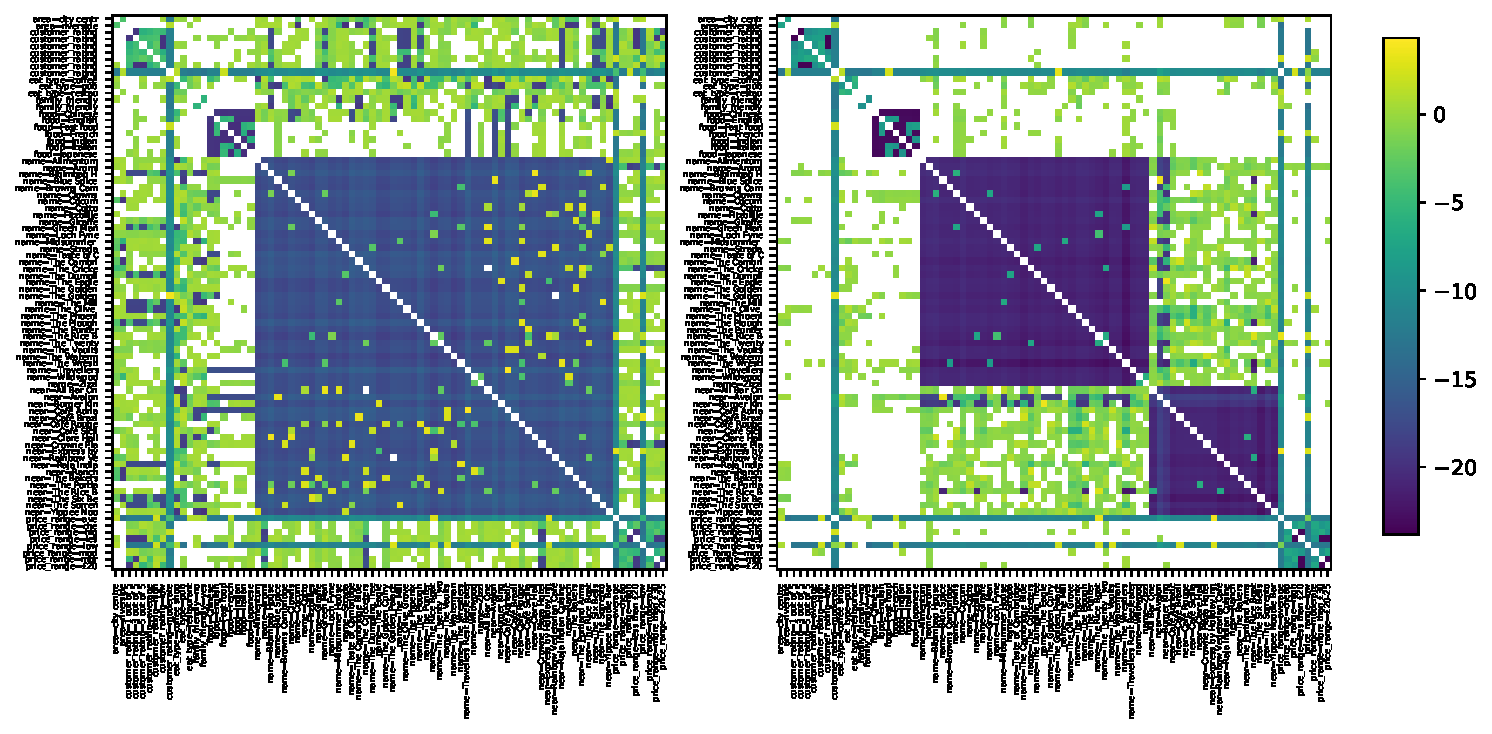
\includegraphics[width=\textwidth]{nlg/heatmap_train.pdf}};
\end{tikzpicture}
\caption{PMI between E2E Challenge attribute-values on the original training data (left) and the union of the training and synthetic data (right). PMI between $(-.25,.25)$ are colored white and suggest relative independence between the two attribute-value pairs. Color blocks on the $x$ and $y$ axis labels correspond to groups of values for the same attribute. E.g., orange are all the values for the \Atr{name}~attribute.}
\label{fig:avpmi}
\end{figure}
